\documentclass[11pt]{amsart}
\usepackage{color,amssymb,amsthm,amstext,latexsym,amsmath,amscd,amsfonts}
\usepackage{tikz}
\usepackage{tcolorbox}
\usepackage{tikz}
\usepackage{tikz-cd}
\usetikzlibrary{calc}

\begin{document}

  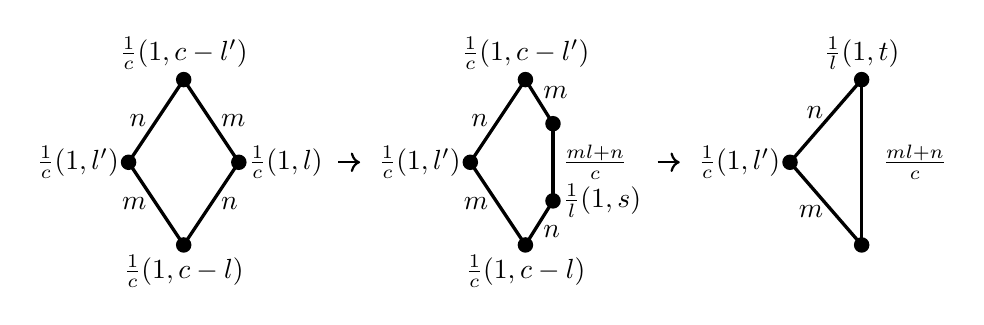
\begin{tikzpicture}[scale=.7]	
  	\coordinate (1A) at (-7.5,3);
				\coordinate (PP1) at (-5,3);
				\fill (PP1) circle (4pt);
				%index 2 points
				\coordinate (PP2) at (-5,0);
				\fill (PP2) circle (4pt);		
				\coordinate (PP3) at (-6,1.5);
				\fill (PP3) circle (4pt);
				\coordinate (PP4) at (-4,1.5);
				\fill (PP4) circle (4pt);		
				\draw[very thick](PP1) -- (PP3);
				\draw[very thick](PP2) -- (PP3);
				\draw[very thick](PP1) -- (PP4);
				\draw[very thick](PP4) -- (PP2);
				\coordinate[label=right:$m$] (AB) at ($(PP1)!0.5!(PP4)$);
				\coordinate[label=left:$n$] (BC) at ($(PP1)!0.5!(PP3)$);
				\coordinate[label=right:$n$] (AB) at ($(PP2)!0.5!(PP4)$);
				\coordinate[label=left:$m$] (BC) at ($(PP2)!0.5!(PP3)$);
				\coordinate[label=above:{$\frac{1}{c}(1,c-l^\prime)$}] (AB) at ($(PP1)$);
				\coordinate[label=below:{$\frac{1}{c}(1,c-l)$}] (AB) at ($(PP2)$);
				\coordinate[label=left:{$\frac{1}{c}(1,l^\prime)$}] (AB) at ($(PP3)$);	
				\coordinate[label=right:{$\frac{1}{c}(1,l)$}] (AB) at ($(PP4)$);


  %%%%%%%%%%%%%%%%%%%%%%%%%%%
      \draw[->, thick] (-2.2,1.5) to (-1.8,1.5);	
    %%%%%%%%%%%%%%%%%%%%%%%%%%

				\coordinate (PP1) at (1.2,3);
				\fill (PP1) circle (4pt);
				%index 2 points
				\coordinate (PP2) at (1.2,0);
				\fill (PP2) circle (4pt);		
				\coordinate (PP3) at (0.2,1.5);
				\fill (PP3) circle (4pt);
				\coordinate (PP4) at (1.7,2.2);
				\fill (PP4) circle (4pt);		
				\coordinate (PP5) at (1.7,.8);
				\fill (PP5) circle (4pt);		
				\draw[very thick](PP1) -- (PP3);
				\draw[very thick](PP2) -- (PP3);
				\draw[very thick](PP2) -- (PP5);
				\draw[very thick](PP1) -- (PP4);
				\draw[very thick](PP4) -- (PP5);
				\coordinate[label=right:$m$] (AB) at ($(PP1)!0.3!(PP4)$);
				\coordinate[label=right:$\quad \quad \quad  \frac{m l +n}{c}$] (AB) at ($(PP3)!0!(PP5)$);
				\coordinate[label=left:$n$] (BC) at ($(PP1)!0.5!(PP3)$);
				\coordinate[label=right:$n$] (AB) at ($(PP2)!0.3!(PP5)$);
				\coordinate[label=left:$m$] (BC) at ($(PP2)!0.5!(PP3)$);
				\coordinate[label=above:{$\frac{1}{c}(1,c-l^\prime)$}] (AB) at ($(PP1)$);
				\coordinate[label=below:{$\frac{1}{c}(1,c-l)$}] (AB) at ($(PP2)$);
				\coordinate[label=left:{$\frac{1}{c}(1,l^\prime)$}] (AB) at ($(PP3)$);	
				\coordinate[label=right:{$\frac{1}{l}(1,s)$}] (AB) at ($(PP5)$);

  %%%%%%%%%%%%%%%%%%%%%%%%%%%
      \draw[->, thick] (3.6,1.5) to (4,1.5);	
    %%%%%%%%%%%%%%%%%%%%%%%%%%  
				\coordinate (PP1) at (7.3,3);
				\fill (PP1) circle (4pt);
				%index 2 points
				\coordinate (PP2) at (7.3,0);
				\fill (PP2) circle (4pt);		
				\coordinate (PP3) at (6,1.5);
				\fill (PP3) circle (4pt);
				\coordinate (PP4) at (7.3,2.2);
				\coordinate (PP5) at (7.3,.8);
				\draw[very thick](PP1) -- (PP3);
				\draw[very thick](PP2) -- (PP3);
				\draw[very thick](PP2) -- (PP5);
				\draw[very thick](PP1) -- (PP4);
				\draw[very thick](PP4) -- (PP5);
				\coordinate[label=right:$\quad \quad \quad  \frac{m l +n}{c}$] (AB) at ($(PP3)!0!(PP5)$);
				\coordinate[label=left:$n$] (BC) at ($(PP1)!0.4!(PP3)$);
				\coordinate[label=left:$m$] (BC) at ($(PP2)!0.4!(PP3)$);
				\coordinate[label=above:{$\frac{1}{l}(1,t)$}] (AB) at ($(PP1)$);
				\coordinate[label=left:{$\frac{1}{c}(1,l^\prime)$}] (AB) at ($(PP3)$);	
  \end{tikzpicture}

\end{document}